\documentclass[a4paper,11pt]{report} 
\usepackage[utf8x]{inputenc}
\usepackage{amsmath} % AMS Math Package
\usepackage{amsthm} % Theorem Formatting
\usepackage{amssymb}	% Math symbols such as \mathbb
\usepackage{graphicx} % Allows for eps images
%\usepackage{multicol} % Allows for multiple columns
%\usepackage[dvips,letterpaper,margin=0.75in,bottom=0.5in]{geometry}
\usepackage{geometry}
\usepackage{booktabs}
\usepackage{enumerate}
\usepackage{verbatim}
\usepackage{fancyhdr}
\usepackage{titlesec}
\usepackage{longtable}
\usepackage{subfigure}
\usepackage{hyperref}
\pagestyle{fancy}
\fancyhf{}
%\fancyhead[LE,RO]{\slshape \rightmark}
\fancyhead[LO,RE]{\slshape \leftmark}
\fancyfoot[C]{\thepage}
%\titleformat{\chapter}%
%[display]{\vspace{2cm}\Large\bfseries}{\Huge\thechapter \ \hrulefill}{0pt}{\vspace{4mm}}%
%{\Large\bfseries\filcenter}

%%%%%%%%%%%%%%%%%%%%%%%%%%%%%%%%%%%%%%%%%%%%%%%%%%%%%%%%%%%%%%%%%%%%%%%%%%%%%%%%%%%%%%%%%%%%%%%%%%%%%%%%%%%%%%%%%%%%%%%%%%%%%%%%%%%%%%%%
						      %Mathematical Commands
%%%%%%%%%%%%%%%%%%%%%%%%%%%%%%%%%%%%%%%%%%%%%%%%%%%%%%%%%%%%%%%%%%%%%%%%%%%%%%%%%%%%%%%%%%%%%%%%%%%%%%%%%%%%%%%%%%%%%%%%%%%%%%%%%%%%%%%%%%
 % Sets margins and page size
%\pagestyle{empty} % Removes page numbers
\makeatletter % Need for anything that contains an @ command 
% \DeclareMathOperator{\Sample}{Sample}
\let\vaccent=\v % rename builtin command \v{} to \vaccent{}
\renewcommand{\v}[1]{\ensuremath{\mathbf{#1}}} % for vectors
\newcommand{\gv}[1]{\ensuremath{\mbox{\boldmath$ #1 $}}} 
% for vectors of Greek letters
\newcommand{\uv}[1]{\ensuremath{\mathbf{\hat{#1}}}} % for unit vector
\newcommand{\abs}[1]{\left| #1 \right|} % for absolute value
\newcommand{\avg}[1]{\left< #1 \right>} % for average
\let\underdot=\d % rename builtin command \d{} to \underdot{}
\renewcommand{\d}[2]{\frac{d #1}{d #2}} % for derivatives
\newcommand{\dd}[2]{\frac{d^2 #1}{d #2^2}} % for double derivatives
\newcommand{\pd}[2]{\frac{\partial #1}{\partial #2}} 
% for partial derivatives
\newcommand{\pdd}[2]{\frac{\partial^2 #1}{\partial #2^2}} 
% for double partial derivatives
\newcommand{\pdc}[3]{\left( \frac{\partial #1}{\partial #2}
 \right)_{#3}} % for thermodynamic partial derivatives
\newcommand{\ket}[1]{\left| #1 \right>} % for Dirac bras
\newcommand{\bra}[1]{\left< #1 \right|} % for Dirac kets
\newcommand{\braket}[2]{\left< #1 \vphantom{#2} \right|
 \left. #2 \vphantom{#1} \right>} % for Dirac brackets
\newcommand{\matrixel}[3]{\left< #1 \vphantom{#2#3} \right|
 #2 \left| #3 \vphantom{#1#2} \right>} % for Dirac matrix elements
\newcommand{\grad}[1]{\gv{\nabla} #1} % for gradient
\let\divsymb=\div % rename builtin command \div to \divsymb
\renewcommand{\div}[1]{\gv{\nabla} \cdot #1} % for divergence
\newcommand{\curl}[1]{\gv{\nabla} \times #1} % for curl
\let\baraccent=\= % rename builtin command \= to \baraccent
\renewcommand{\=}[1]{\stackrel{#1}{=}} % for putting numbers above =
\newtheorem{prop}{Proposition}
\newtheorem{thm}{Theorem}[section]
\newtheorem{lem}[thm]{Lemma}
\theoremstyle{definition}
\newtheorem{dfn}{Definition}
\theoremstyle{remark}
\newtheorem*{rmk}{Remark}
\usepackage[italian]{babel}
\usepackage{graphicx}
\usepackage{latexsym}
\usepackage{verbatim} % commenti estesi
\newcommand{\p}[2]{ \frac{ \partial #1}{ \partial #2}} %derivata partiale
\newcommand{\lap}{\nabla^2} %laplaciano
\newcommand{\ham}{\mathcal{H}} % Simbolo dell'hamiltoniana
\newcommand{\rint}{\int_\mathbb{R}} % Integrale su R
\newcommand{\modq}[1]{| #1|^2} % Modulo quadro di ``argomento''
\newcommand{\navg}[2]{\left< #1 ^{#2} \right>} %media di ``arg''^n
\newcommand{\con}[1]{\overline{#1}} %coniugato con la barra
\newcommand{\ih}{\frac{i}{\hbar}} % i/h tagliato
\newenvironment{sistem}%
{\left\lbrace\begin{array}{@{}l@{}}}%
{\end{array}\right.}



\title{Relazioni di Laboratorio di Fisica Computazionale}
\author{Carlo Sana}
\begin{document}
\maketitle
\tableofcontents
\chapter{Integrazione numerica}
Si vuole calcolare il valore dell'integrale definito di una funzione reale di variabile reale in una dimensione:
$$
 	I \ = \ \int_{x_{min}}^{x_{max}} f(x) \, dx
$$
%% BRUTTO
I metodo di integrazione numerica implementati si suddividono in metodi deterministici e  metodi Monte Carlo.
\section{Metodi deterministici}
Le prime routine di integrazione deterministica sono un'implementazione delle formule di Newton-Cotes (al primo e secondo ordine) e del metodo delle quadrature gaussiane.\\
Per aumentare la precisione del calcolo, il dominio di integrazione viene suddiviso in sottointervalli.
La larghezza di ogni intervallo è uniforme ed è possibile scegliere il numero di intervalli in cui
si vuole dividere il dominio di integrazione prima di chiamare le funzioni.
Per ottenere la stima dell'integrale è necessario sommare le stime degli integrali ottenute per i sottointervalli.\\
Nel nostro caso $n$ sarà il numero di sottointervalli. Definiamo così in modo naturale una partizione dell'insieme di integrazione:
$$
	h \ = \frac{x_{max} - x_{min}}{ n} \qquad \Longrightarrow \qquad a_i = x_{min} + i h  \qquad
	\mbox{ per } \ i = 0,1,....,n 
$$
Nel caso gli estremi di integrazione sono scambiati, ossia $x_{min} > x_{max}$, l'integrazione avviene comunque correttamente,
visto che in questo caso $h$ sarà negativo.
\subsection{Newton-Cotes}
Le formule di Newton-Cotes si ottengono interpolando la funzione integranda con polinomi di Lagrange.
Il polinomio di Lagrange j-esimo di grado n è definito come:
$$
	l_j^n (x)\ = \ \prod_{i = 0, i \ne j}^{n} \frac{x-x_i}{x_j - x_i}
$$
	Come si può vedere è un polinomio di grado n, definito in base alla partizione scelta per l'intervallo, con la proprietà:
$$
	l_j^n ( x_i) = \delta_{ij}
$$
E' ora immediato costruire un polinomio $P(x)$ tale che $ P(x_i) = f(x_i) \ \ \forall \   0<i<n$.\\
Questo polinomio è il seguente:
$$
	P(x) = \sum_{i = 0}^n f(x_i) l_i^n(x)
$$
La stima dell'integrale diventa così:
$$
 I \ = \ \int_{x_{min}}^{x_{max}} P(x) \, dx \ \ = \ \int_{x_{min}}^{x_{max}} \sum_{i = 0}^n f(x_i) l_i^n(x)  \ =  \ \sum_{i = 0}^n f(x_i) \omega_i 
$$
 Si dimostra inoltre che, con un cambio di variabile:
 $$
 \omega_j = \int_{x_{min}}^{x_{max}} l_i^n(x) \,dx  = \int_{0}^{n} \prod_{i = 0 \ i \ne j}^n \frac{z-i}{j-i}\,dz 
$$
indipendente dall'intervallo di integrazione.\\
Questa è ovviamente una stima dell'integrale e si dimostra che l'errore, utilizzando $n+1$ punti è uguale a :
$$
 E_n = \frac{1}{(n+1)!} \int_{x_{min}}^{x_{max}} f^{n+1}(\xi) \prod_{i = 0}^n {(x-x_i)} \, dx 
 $$
%\leq \frac{1}{(n+1)!}(x_{max}-x_{min})\ max(f^{n+1}(\xi),[x_{min},x_{max}]

 dove $\xi$ è un punto interno all'intervallo. L'errore è facilmente sovrastimabile, valutando il massimo della derivata $n+1$-esima all'interno dell'intervallo. L'errore sulla stima dell'integrale,
però, non viene calcolato dalla routine d'integrazione. Ciò deriva dal fatto che esso è stimabile analiticamente,
essendo necessario solo calcolare la derivata dell'integranda e valutarne il massimo nell'intervallo.

\subsubsection{Newton-Cotes:1°ordine}
Questo metodo consiste nell'approssimare la funzione fra due punti $a_i$ e $a_{i+1}$ con un segmento.
L'area si ottiene calcolando l'area del trapezio sotteso da questo segmento, oppure applicando le formule di Newton-Cotes, ponendo $ n = 1$: 
$$
\omega_0 \ = \ \frac{1}{2} \qquad \omega_1 \ = \ \frac{1}{2}
$$
In questo caso la stima analitica dell'errore diventa:
$$
| E_1(f) |  \ = \ \frac{h^3}{12} \ f''(\xi) \leq \  \frac{h^3}{12} \max \left[ f''(x), x \in [x_{min},x_{max}] \right]
$$
Questa formula vale nel caso venga considerato un solo intervallo. Nel nostro caso, l'intervallo è stato suddiviso in $n$ sottointervalli. Una buona sovrastima dell'errore è dunque:
$$
| E_1(f) |  \ \leq \ \frac{h^2}{12}\left( x_{max} - x_{min} \right) \max \left[ f''(x), x \in [x_{min},x_{max}] \right]
$$
\subsection{Newton-Cotes:2°ordine}
In questo caso, l'approssimazione viene fatta con polinomi di grado 2, ossia parabole.
I "pesi" $\omega_i$ valgono:
$$
	\omega_0 = \frac{1}{6} \qquad  \omega_1 = \frac{2}{3} \qquad \omega_2 = \frac{1}{6}
$$
La stima dell'errore si può scrivere come:
$$
|E_2 (f) | \ = \  \frac{h^5}{90} \ f^4(\xi) \leq \ \frac{h^5}{90} \ max \left[ f^4( x), x \in [x_{min},x_{max}] \right]
$$
Come nel caso precedente, nel caso di $n$ sottointervalli, la sovrastima corretta diviene:
$$
|E_2 (f) | \ \leq \ \frac{h^4}{90} \left( x_{max} - x_{min} \right) \ max \left[ f^4( x), x \in [x_{min},x_{max}] \right]
$$

\subsection{Quadrature gaussiane}
Nel caso delle quadrature gaussiane, i punti della partizione non vengono più scelti equidistanti,
ma vengono scelti in maniera più opportuna: sono gli zeri del polinomio ortogonale scelto.\\
E' fondamentale l'uso di polinomi ortogonali in un certo intervallo $[a,b]$ con il peso $\omega(x)$:
$$
	\int_a^b \omega(x)\ P_n{(x)} \ P_m{(x)} \ = \ \delta_{m,n}
$$
Si può dimostrare che la stima dell'integrale è:
$$
 I \ = \  \int_a^b f(x) \ = \ \sum_{i=0}^n \omega_i f(x_i)
$$
dove $\omega_i$, nel caso dei polinomi di Legendre, sono gli stessi pesi definiti per i polinomi di Lagrange costruiti sull'insieme degli zeri
del polinomio di Legendre considerato. Considerando che un polinomio ortogonale di grado $n$ in $[a,b]$ ha $n$ zeri in $[a,b]$, anche i polinomi
di lagrange saranno di grado $n$. Inoltre $x_i$ sono gli zeri del polinomio ortogonale considerato.
Gli zeri del polinomio sono stati inseriti manualmente, lasciando però al calcolatore il compito di calcolarne il valore in virgole mobile,
per aumentarne la precisione.
All'interno dell'algoritmo, è necessario effettuare un cambio di variabile in modo da mappare l'intervallo
di integrazione nell'intervallo in cui il polinomio è ortogonale. Nel nostro caso tale intervallo è $[-1,1]$,
dato che è stato usato un polinomio di Legendre.\\
Tale cambio di variabile è:
$$
	x' \ = \ 2 \frac{x - x_{min} }{x_{max}-x_{min}} - 1 \qquad dx'  \ = \ 2 \frac{dx}{x_{max}-x_{min}}
$$
\subsection{Utilizzo}
Il programma ``integral'' si occupa di utilizzare le librerie appena discusse per stimare il valore dell'integrale di una funzione, confrontando i
tre metodi discussi sopra. Per testare le routine ho utilizzato come funzioni da integrare:
$$
  f_1 (x) \ = log ( 1+x) \quad \Rightarrow \quad \mbox{primitiva }\ -x + log(1 + x) + x log(1 + x)
$$
$$
 f_2 (x) \ = \ 	x^9 - x^7 + 3 \quad \Rightarrow \quad \mbox{primitiva }\  \frac{x^{10}}{10} - \frac{x^8}{8} + 3x
$$
In questo modo si è potuto confrontare i tre metodi di integrazione con il valore vero dell'integrale, valutandone
lo scostamento dal valore vero e confrontandolo con la stima dell'errore calcolata analiticamente.
È riportata nella tabella seguente una serie di risultati ottenuti variando il numero di intervalli, ma mantenendo costanti gli estremi di integrazione.
In questo caso l'intervallo di integrazione è stato $[1,2]$.
La prima tabella si riferisce alla funzione integranda di tipo logaritmico, la seconda a quella di tipo polinomiale.
La stima analitica dell'errore è stata calcolata valutando il massimo della derivata in tutto l'intervallo di integrazione.
Questa risulta essere una sovrastima della stima dell'errore. Tali valori sono stati calcolati con \emph{Wolfram Mathematica} e risultano essere:
\begin{center}
\begin{longtable}{lcr}
 \toprule
 funzione & Max $f'$ & Max $f^4$ \\
 \midrule
 $f_1$ (Log)  &  0.5 & -0.0740742 \\
 $f_2$ (Poly) &	1856 & 90048 \\
\end{longtable}
\end{center}

%%%
%%% MANCANO LE DIDASCALIE AI GRAFICI!

%%% CERCA COME RIPORTARE L' INTESTAZIONE SE CAMBI Pagina
%%% LOgaritmo
\subsubsection{Newton-Cotes I: Logaritmo}
\begin{figure}[h]
\includegraphics[width=0.7\columnwidth,angle=-90]{plot_trap_log.eps}
\caption{Errori per Newton-Cotes I: Logaritmo}
\end{figure}
\begin{center}
\begin{longtable}[h]{lcr}
\toprule
Log &  \\
\midrule
Numero intervalli & Newton-Cotes I & Stima analitica errore  \\
\midrule
10 &	  1.388645e-04  	 & 4.166667e-04 \\ 
20 &	 3.472070e-05  		 & 1.041667e-04 \\ 
40 &	 8.680460e-06  		 & 2.604167e-05 \\ 
80 &	 2.170133e-06  		 & 6.510417e-06 \\ 
160 &	 5.425343e-07  		 & 1.627604e-06 \\ 
320 &	 1.356337e-07  		 & 4.069010e-07 \\ 
640 &	  3.390842e-08  	 & 1.017253e-07 \\ 
1280 &	  8.477104e-09  	 & 2.543132e-08 \\ 
2560 &	  2.119278e-09  	 & 6.357829e-09 \\ 
5120 &	  5.298200e-10  	 & 1.589457e-09 \\ 
10240 &	  1.324560e-10  	 & 3.973643e-10 \\ 
20480 &	  3.310918e-11  	 & 9.934107e-11 \\ 
40960 &	  8.281043e-12  	 & 2.483527e-11 \\ 
81920 &	  2.071121e-12  	 & 6.208817e-12 \\ 
\end{longtable}
%% LOG 222222222222222
\end{center}
Da questo confronto si nota come l'errore scala come previsto analiticamente e rimane sempre inferiore alla stima fatta analiticamente.

\subsubsection{Newton-Cotes II: Logaritmo}
\begin{figure}[h]
\includegraphics[width=0.7\columnwidth,angle=-90]{plot_simp_log.eps}
\caption{Errori per Newton-Cotes II: Logaritmo}
\end{figure}

  \begin{center}
  \begin{longtable}[h]{lcr}
\toprule
Log & & \\
\midrule
Numero intervalli & Newton-Cotes II & Stima analitica errore  \\
\midrule
10 & 	  -6.101824e-09  	 & -8.230467e-08 \\  
20 & 	  -3.816787e-10  	 & -5.144042e-09 \\  
40 & 	  -2.386025e-11  	 & -3.215026e-10 \\  
80 & 	  -1.491696e-12  	 & -2.009391e-11 \\  
160 & 	  -9.336976e-14  	 & -1.255870e-12 \\  
320 & 	  -6.217249e-15  	 & -7.849185e-14 \\  
640 & 	  -2.220446e-16  	 & -4.905740e-15 \\  
1280 & 	  -1.443290e-15  	 & -3.066088e-16 \\  
2560 & 	  -6.661338e-16 	 & -1.916305e-17 \\  
5120 & 	  -2.664535e-15 	 & -1.197691e-18 \\  
10240 &  1.443290e-15  	 & -7.485566e-20 \\  
20480 &  2.220446e-15  	 & -4.678479e-21 \\  
40960 &  2.220446e-15  	 & -2.924049e-22 \\  
81920 &  -3.108624e-15   	&-1.827531e-23 \\  
\bottomrule
\end{longtable}
\end{center}
in questo caso invece l'errore scala correttamente fino a quando raggiunge il valore di $ 10^{-15}/ 10^{-16}$. A quel punto smette di
diminuire all'aumentare degli intervalli considerati ed inizia ad oscillare, cambiando anche di segno.

\subsubsection{Quadrature gaussiane: Logaritmo}
\begin{center}
% LOG GAUSSIANA
\begin{longtable}[h]{lr}
\toprule
Log & \\
\midrule
Numero intervalli & quadratura gaussiana \\
10 &	2.220446e-16 \\
20 &	2.220446e-16 \\
40 &	2.220446e-16 \\ 
80 &	2.220446e-16 \\
160 &	5.551115e-16 \\ 
320 & 	1.221245e-15 \\
640 &	-3.330669e-16 \\ 
1280 &	1.332268e-15 \\
2560 &	 -6.661338e-16 \\
5120 &	 -2.775558e-15 \\ 
10240 &	-1.443290e-15 \\ 
20480 &	 -2.220446e-15 \\
40960 &	 -2.109424e-15 \\ 
81920 &	2.997602e-15 \\
\midrule

\bottomrule
\end{longtable}
\end{center}
\subsubsection{Newton-Cotes I: Polinomio}
\begin{figure}[h]
\includegraphics[width=0.7\columnwidth,angle=-90]{plot_trap_poly.eps}
\caption{Errori per Newton-Cotes I: Polinomio}
\end{figure}

\begin{center}
% POLI 111111111111111111
\begin{longtable}[h]{lcr}
\toprule
Poly & & \\
\midrule
Numero intervalli & Newton-Cotes I & Stima analitica errore  \\
\midrule
10 &	  1.541035e+00  	 & 1.546667e+00 \\  
20 &	  3.860018e-01  	 & 3.866667e-01 \\  
40 &	  9.654698e-02  	 & 9.666667e-02 \\  
80 &	  2.413966e-02  	 & 2.416667e-02 \\  
160 &	  6.035096e-03  	 & 6.041667e-03 \\  
320 &	  1.508785e-03  	 & 1.510417e-03 \\  
640 &	  3.771970e-04  	 & 3.776042e-04 \\  
1280 &	  9.429930e-05  	 & 9.440104e-05 \\  
2560 &	  2.357483e-05  	 & 2.360026e-05 \\  
5120 &	  5.893707e-06  	 & 5.900065e-06 \\  
10240 &	  1.473427e-06  	 & 1.475016e-06 \\  
20480 &	  3.683565e-07  	 & 3.687541e-07 \\  
40960 &	  9.208941e-08  	 & 9.218852e-08 \\  
81920 &	  2.302234e-08  	 & 2.304713e-08 \\  
\bottomrule
\end{longtable}
\end{center}
in questo caso l'andamento è simile al caso della funzione logaritmica interpolata con il metodo dei trapezi.
Si può notare che in questo caso la differenza fra l'errore stimato e l'errore di integrazione è molto piccola.
In ogni caso l'errore stimato è sempre maggiore dell'errore di integrazione.\\
%%% POLINOMIO 2222222222222222222
\subsubsection{Newton-Cotes II: Polinomio}
\begin{figure}[h]
\includegraphics[width=0.7\columnwidth,angle=-90]{plot_simp_poly.eps}
\caption{Errori per Newton-Cotes II: Polinomio}
\end{figure}

\begin{center}
\begin{longtable}[h]{lcr}
\toprule
Poly & & \\
\midrule
Numero intervalli & Newton-Cotes II & Stima analitica errore  \\
\midrule
10 & 	  9.908609e-04 & 	  1.000533e-01 \\  
20 & 	  6.203492e-05 & 	  6.253333e-03 \\  
40 & 	  3.878841e-06 & 	  3.908333e-04 \\  
80 & 	  2.424535e-07 & 	  2.442708e-05 \\  
160 & 	  1.515373e-08 & 	  1.526693e-06 \\  
320 & 	  9.471250e-10 & 	  9.541829e-08 \\  
640 & 	  5.921663e-11 & 	  5.963643e-09 \\  
1280 & 	  3.652190e-12 & 	  3.727277e-10 \\  
2560 & 	  1.847411e-13 & 	  2.329548e-11 \\  
5120 & 	  4.263256e-14 & 	  1.455968e-12 \\  
10240 & -1.705303e-13  	 & 9.099798e-14 \\  
20480 & 4.263256e-14  	 & 5.687374e-15 \\  
40960 & -3.552714e-13 	 & 3.554608e-16 \\  
81920 & 4.263256e-14  	 & 2.221630e-17 \\  

\bottomrule
\end{longtable}
\end{center}
anche in questo caso l'andamento è simile alla funzione logaritmica, anche se l'errore inizia ad oscillare ad un valore di $10^{-13}/10^{-14}$.  
\subsubsection{Quadrature gaussiane: Polinomio}
\begin{center}
\begin{longtable}[h]{lr}
\toprule
Poly & \\
\midrule
Numero intervalli & quadratura gaussiana  \\
10	&0.000000e+00 \\
20&	0.000000e+00 \\ 
40&	1.421085e-14 \\
80&	1.421085e-14 \\
160&	2.842171e-14 \\
320&	0.000000e+00 \\
640&	2.842171e-14 \\
1280&	-2.842171e-14 \\ 
2560&	2.842171e-14 \\
5120&	-2.842171e-14 \\ 
10240&	1.705303e-13 \\
20480&	-4.263256e-14 \\
40960&	3.552714e-13 \\ 
81920&	-2.842171e-14 \\
\midrule

\bottomrule
\end{longtable}
 
\end{center}
Dall'analisi di questi dati è possibile trarre alcune conclusioni riguardo i diversi metodi di integrazione deterministica utilizzati.
È banale notare come la precisione dell'integrazione con le formule di Newton-Cotes al II° ordine sia molto maggiore di quelle al I° ordine, al prezzo di un costo computazionale ovviamente maggiore.
Inoltre, si nota come l'errore scali nella maniera prevista fino a quando diventa troppo ``piccolo'' e inizia ad oscillare attorno a zero.
Questo può essere dovuto alla precisione con cui sono salvati i numeri nel calcolatore, nonostante siano state usate variabili di tipo \emph{double} in tutto il codice.
In ogni caso, si può notare come gli errori abbiano un andamento asintotico in accordo con la previsione teorica prima che si facciano sentire gli errori di approssimazione del calcolatore.
 
%%
%% COMPLETA LA RIFLESSIONE
%% 

\section{Metodi Monte Carlo}
\label{sec:Monte Carlo}
Per metodi Monte Carlo si intendono algoritmi basati sulla generazione di dati in modo non deterministico.
Generalmente vengono utilizzate sequenze di numeri \emph{casuali} o \emph{pseudocasuali} che verranno analizzate e 
manipolate opportunamente all'interno dell'algoritmo in modo da ottenere una risposta statisticamente significativa al problema.\\
Il metodo più generale per l'integrazione Monte Carlo consiste nell'utilizzare un generatore di numeri \emph{pseudocasuali} con distribuzione
di probabilità piatta. La formula che restituisce il valore dell'integrale è:
$$
    I \ = \ \int_{x_{min}}^{x_{max}} f(x) \, dx \ \simeq \ \frac{1}{n} \sum_i \ f(x_i) \ + \ o\left(\frac{1}{\sqrt{n}}\right)
$$
dove gli $x_i$ sono estratti tra $x_{min}$ e $x_{max}$. $n$ indica il numero di numeri pseudocasuali estratti.\\
Questo metodo ha lo svantaggio di ritornare valori poco precisi nel caso la funzione integranda sia estremamente piccata intorno a un punto e
zero nel resto dell'intervallo. Questo deriva dal fatto che il generatore estrae numeri in maniera ``cieca'', senza tenere conto della funzione.\\
È possibile migliorare questo aspetto, attraverso il metodo del campionamento di importanza. Esso consiste nel generare numeri secondo una distribuzione
di probabilità nota e il più possibile simile alla funzione integranda. 
$$
 I \ = \ \int_{x_{min}}^{x_{max}} f(x) \, dx \ = \ \int \frac{f(x)}{g(x)} \left( g(x) dx \right) \ \simeq \ \frac{1}{n} \sum_i \ \frac{f(x_i)}{g(x_i)} 
$$
Data la natura probabilistica dell'algoritmo, è necessario utilizzare un approccio statistico per ottenere un errore associato al valore dell'integrale.
Abbiamo quindi:
$$
  \sigma^2 = <{f(x)}^2> - <{f(x)}>^2 = \int (f(x) - I)^2 \ dx  
$$
Nel caso utilizziamo il metodo campionamento di importanza:
$$
\sigma^2 \ = \ <{\left(\frac{f(x)}{g(x)}\right)}^2> - <{\frac{f(x)}{g(x)}}>^2 = \int \left(\frac{f(x)}{g(x)} - I\right)^2 \ dx  
$$
si deduce così che nel caso $ g(x) \ \simeq \ \frac{f(x)}{I}$ la varianza tende a zero.
La difficoltà risiede, però, nel riuscire a creare un generatore di numeri \emph{pseudocasuali} secondo una distribuzione di probabilità a piacere.
\subsubsection{Generatori di numeri pseudocasuali}
Nel nostro caso ci occuperemo di calcolare il valore dei momenti gaussiani attraverso la tecnica esposta precedentemente. \\
Nel programma ``importanza'' sono confrontate tre diverse distribuzioni di probabilità per calcolare il secondo e il quarto momento gaussiano:
\begin{align*}
\nonumber
P_{flat}(x) &= 1 \quad \mbox{per} \quad x_{min} < x < x_{max}\\
\nonumber
P_{root}(x) &= \frac{2}{\sqrt{\pi}} e^{-x} \sqrt{x}\\
\nonumber
P_{gauss}(x) &= \frac{2}{\sqrt{\pi}} e^{-x^2}
\end{align*}
La prima distribuzione è generata dalle funzioni in \emph{ranlxd.h} ed è stata assunta come corretta. Questa assunzione è necessaria visto che le altre
due distribuzioni saranno generate a partire da essa. La distribuzione $P_{gauss}(x)$ è generate con il seguente cambio di variabile, a partire
da due variabili casuali ``piatte'':
$$
\hat{x_1} \, , \hat{x_2} \qquad 0 \leq x_1 , x_2 \leq 1
$$
\begin{align*}
 \nonumber
 {y_1}^2 \ &= \ - \log(1-x_2) \sin^2\left(\frac{\pi}{2} x_1 \right) \\ 
 \nonumber
 {y_2}^2 \ &= \ - \log(1-x_2) \cos^2\left(\frac{\pi}{2}x_1 \right) 
\end{align*}
La distribuzione $P_{root}(x)$ invece si ottiene con il seguente cambio di variabile:
\begin{align*}
 \nonumber
 \hat{x_1} \quad P(x_1) \ &= \frac{2}{\pi} e^{-x_1^2} \\
 \hat{x_2} \quad P(x_2) \ &= e^{-x_2}
\end{align*}
\begin{align*}
 y_1 \ &= x_1^2 + x_2 \\
 y_2 &= x_2
\end{align*}
A questo punto la distribuzione di probabilità ottenuta è:
$$
P(y_1,y_2) \ = \ \frac{2}{\sqrt{\pi}} e^{-\left(y_1^2 + y_1\right)}\frac{1}{2\sqrt{y_1 -y_2}} 
$$
La distribuzione ricercata si ottiene integrando sulla seconda variabile. Ciò equivale ad utilizzare esclusivamente la prima variabile $y_1$
come variabile casuale.
\subsubsection{Confronto tra le distribuzioni}
Le diverse distribuzioni sono state confrontate nel calcolare il secondo e il quarto momento gaussiano:
\begin{align*}
\mu_2(x) \ &= \ \int_{-\infty}^{+\infty} x^2 \frac{1}{\sqrt{\pi}} e^{-x^2}  = \frac{1}{2}\\
\mu_4(x) \ &= \ \int_{-\infty}^{+\infty} x^4  \frac{1}{\sqrt{\pi}} e^{-x^2} = \frac{3}{4}
\end{align*}
Si può prevedere che la distribuzione $P_{root}$ fornisca un errore minore, dato che è più simile alle funzioni integrande.\\

\begin{figure}[h]
\includegraphics[width=0.6\columnwidth,angle=-90]{importanza_integrale.eps}
\caption{Confronto tra il valore dell'integrale con le diverse distribuzioni.}
\end{figure}
\begin{center}
 \begin{longtable}[htb]{lccr}
  \toprule
  Valore $\mu_2$ & 0.5 & & \\
  \midrule
  N & $P_{flat}$ & $P_{gauss} $  & $P_{root}$ \\
  \midrule
1000   & 0.402414	& 0.509921 	& 0.520847  \\
2000   & 0.478750	& 0.500909 	& 0.503343 \\
4000   & 0.559025	& 0.516745 	& 0.493403 \\
8000   & 0.529128	& 0.508603 	& 0.496762 \\
16000  & 0.528902	& 0.497904 	& 0.500056 \\
32000  & 0.527839	& 0.500956 	& 0.501474 \\
  \bottomrule
  \end{longtable}
\end{center}

\begin{center}
 \begin{longtable}[ht]{lccr}
  \toprule
  Valore $\mu_2$ & 0.75 & & \\
  \midrule
  N & $P_{flat}$ & $P_{gauss} $  & $P_{root}$ \\
  \midrule
1000   & 0.819771 & 	0.639290&0.761542    \\
2000   & 0.734319 & 	0.679399&0.735870   \\
4000   & 0.710013 & 	0.771816&0.742201   \\
8000   & 0.824491 & 	0.719916&0.741778   \\
16000  & 0.788585 & 	0.748977&0.748735   \\
32000  & 0.718003 & 	0.743117&0.751811   \\
  \bottomrule
  \end{longtable}
\end{center}

Da questo grafico si nota come l'utilizzo di distribuzioni non piatte porti a una significativa diminuizione dell'errore. Inoltre, come ci aspettavamo,
la distribuzione $P_{root}$ è quella che fornisce una stima migliore dell'integrale, a parità di numeri estratti.
È necessario controllare che l'algoritmo fornisca risultati con l'andamento asintotico atteso analiticamente come verifica della sua correttezza.
Si può dimostrare che l'errore di integrazione è asintotico a $ \frac{1}{\sqrt{n}}$. In ordinata è stato quindi posto:
$$
 \frac{ \sigma}{I} \simeq  \ \frac{A}{\sqrt{n}} \quad  \longrightarrow \quad y = \frac{ \sigma}{I} \sqrt{n}\simeq \ A 
$$
 Per questo motivo ci aspettiamo che nel grafico i punti siano allineati all'incirca su rette orizzontali. Il valore dell'ordinata indica, dunque,
 il coefficiente dell'andamento asintotico dell'errore. Da ciò possiamo dedurre che la distribuzione $P_{root}$, avendo come valore di $A$ minore,
 è quella che fornisce un valore dell'integrale più preciso.
\begin{figure}[h]
\includegraphics[width=0.6\columnwidth,angle=-90]{importanza_noise.eps}
\caption{Andamento asintotico del ``rumore''.}
\end{figure}


\chapter{Oscillatore armonico}
Si è risolto l'oscillatore armonico quantistico monodimensionale attraverso l'utilizzo degli integrali di cammino sul reticolo.
È stato scelto un approccio non-determnistico attraverso l'integrazione Monte Carlo.\\
Il tempo è stato discretizzato in $N$ istanti e, ponendo $T$ come istante finale e $0$ come istante iniziale,
abbiamo il passo reticolare temporale $ a = \frac{T}{N}$ .
\section{Integrali di cammino}
Nel formalismo del \emph{path integral} sul reticolo è fondamentale introdurre il concetto di azione.
Nel nostro caso sarà importante la definizione di azione euclidea:
$$
 S_E  \ = \ a \sum_{i=0}^{n-1} \mathcal{L}_E(x_i,x_{i+1})
$$
dove
$$
\mathcal{L}_E(x_i,x_{i+1}) \ = \ \frac{m}{2} \left( \frac{x_{i+1} -x_{i}}{a} \right)^2 + \frac{1}{2}V(x_i)  +\frac{1}{2}V(x_{i+1})
$$
 Si ricava un equivalente alla funzione di partizione classica definita come: 
$$
 Z_a (0,T) =  \ \left( \frac{m}{2 \pi a}\right)^{N/2} \int \prod_{i=1}^{N-1} dx_i \ e^{-S_E}
$$
e il correlatore fra due operatori di posizione è uguale a:
$$
 C( | l -k|) \ = \ \langle x_l \ x_k \rangle  \ = \  \frac{ \int \prod_{i=1}^{N-1} dx_i \ x_l \ x_k \ e^{-S_E}}{Z_a}
$$
Si dimostra che:
$$
 C( | l -k|) \ = \  \langle x_l \ x_k \rangle \ = \ 2 | \langle \tilde{E_0} | \hat{x} | \tilde{E_1} \rangle  |^2 \ \ \exp{\left( - \frac{N a}{2} \left( \tilde{E_1}-\tilde{E_0} \right) x \right)} \cosh \left[ a \left( \frac{N}{2} - | l - k | \right) (\tilde{E_0} -\tilde{E_1}) \right]  
$$
$$ 
\langle \tilde{E_0} | \hat{x} | \tilde{E_1} \rangle  = \frac{1}{\sqrt{2  m \bar{\omega}}}
$$
dove è stato posto
$$
 \bar{\omega}^2  \ = \  \omega^2 \left(1 + \frac{a^2 \omega^2}{4} \right) \qquad a \tilde{\omega} \ = \ ln \left( 1 + a \bar{\omega} + \frac{a^2 \omega^2}{2} \right) \qquad \tilde{E_n} \ = \  \tilde{\omega}\left( n + \frac{1}{2} \right) 
$$
Nel nostro caso, si è posto $ N \ = \ 32 $, ma l'algoritmo è indipendente da $N$.\\
Ciò che viene calcolato dall'algoritmo sono i valor medi $\langle x_l \ x_k \rangle $ per ogni valore di $ | l - k| $ e i relativi errori.
Da essi siamo in grado di estrarre il valore di $ \langle E_0 | \hat{x} | E_1 \rangle $ e $ \tilde{E_1}-\tilde{E_0} $.
Gli errori sulle grandezze secondarie sono stati calcolati con il metodo \emph{cluster jackknife}.
\section{Algoritmo Metropolis}
Per calcolare $\langle x_l \ x_k \rangle $ con un metodo Monte Carlo è necessario riuscire ad estrarre numeri casuali secondo la \emph{pdf} $ e^{-S_E}$.
L'algoritmo \emph{Metropolis-Hastings} permette di estrarre numeri casuali secondo una \emph{pdf} qualsiasi a partire da un generatore ``piatto''.\\
Più in generale esso permette, dato uno spazio di configurazioni $S$ e una \emph{pdf} $ P(s) : S \rightarrow \mathbb{R}$, di estrarre
configurazioni del sistema compatibili con la \emph{pdf} voluta.Ciò è particolarmente utile in quanto non è sempre possibile trovare un cambio
di coordinate che permette di ottenere la distribuzione voluta a partire da una distribuzione piatta,
come è stato fatto nell'integrazione Monte Carlo discussa in \ref{sec:Monte Carlo}.\\
L'algoritmo si basa sul metodo del rigetto. Poniamo di avere uno stato $s$ nello spazio delle configurazioni. A questo punto:
\begin{itemize}
  \item si estrae una nuova configurazione del sistema $s'$ con il generatore di numeri random ``piatto''.
  \item si calcola il rapporto $ \frac{P(s')}{P(s)}$.
  \item si accetta il nuovo stato estratto $s'$ con probabilità pari a $ min\left[ 1,\frac{P(s')}{P(s)} \right]$.
\end{itemize}
Si dimostra che gli stati del sistema vengono estratti con la \emph{pdf} da noi cercata,
a patto di attendere che il sistema si termalizzi.
Questo è dovuto al fatto che la \emph{pdf} di estrazione delle configurazioni approssima la distribuzione $P$ solo in regime asintotico.
\subsubsection{Implementazione dell'algoritmo Metropolis all'oscillatore armonico}
Nel caso dell'oscillatore armonico la \emph{pdf} ricercata è $ e^{-S_E}$, opportunamente normalizzata.
Inoltre, lo spazio delle configurazioni coincide con $\mathbb{R}^N$, dove $N$ è il numero di coordinate. D'ora in poi per $\hat{e_i}$ si intenderà l'$i$-esimo vettore
della base canonica in $\mathbb{R}^N$.
In questo caso, grazie alla presenza dell'esponenziale nella \emph{pdf},
il rapporto $ \frac{P(s')}{P(s)}$ si semplifica ulteriormente, e l'algoritmo diventa:
\begin{itemize}
 \item si estrae una nuova configurazione del sistema $\vec{x'}$: esso corrisponde a $\vec{x} + \left(\delta \ rand() - \frac{\delta}{2}\right)\hat{e_i}$.
  \\
  $rand()$ è un numero casuale fra 0 e 1, $\delta$ è un parametro per regolare la traslazione (in questo caso è uguale a 2).
  È importante notare che viene cambiata una coordinata alla volta per ogni passo del Metropolis.
 \item si calcola $\Delta S_E \ = \ S_E(\vec{x}') -S_E(\vec{x})$
%  \item si accetta il nuovo stato con probabilità $ min \ \left[1,e^{- \Delta S_E}\right]$
\end{itemize}
Dato che ad ogni passo del Metropolis viene modificata solo una coordinata, è possibile valutare $\Delta S_E$ in una forma più efficiente come costo computazionale.
\begin{equation*}
\Delta S_E \ = \ a[\mathcal{L}(x_{i-1},x'_{i})+\mathcal{L}(x'_{i},x_{i+1})-\mathcal{L}(x_{i-1},x_{i})-\mathcal{L}(x_{i},x_{i+1})]    
\end{equation*}
\subsubsection{Inizializzazione e termalizzazione dell'algoritmo}
Prima che l'algoritmo Metropolis riesca a generare configurazioni del sistema con la \emph{pdf} voluta, è necessario che entri in regime asintotico.
È possibile stimare il tempo di termalizzazione dell'algoritmo graficando l'andamento dell'azione euclidea $S_E$ in funzione del tempo markoviano.\\
In questo caso si è scelto di inizializzare il la configurazione di partenza in modo che tutte le variabili fossero inizializzate a zero: ossia è stato fatta una
\emph{cold start}.
\begin{center}
  \begin{figure}[h]
    \includegraphics[width=0.6\columnwidth,angle = -90]{action_cold.eps}
    \caption{Andamento dell'azione euclidea in funzione del numero di sweeps.}
  \end{figure}
\end{center}
Come si vede nel grafico, l'azione parte da zero e cresce velocemente. Dopo circa cento \emph{sweeps} si può vedere come l'algoritmo sia già in un regime asintotico.
All'interno del programma è stato scelto come tempo di termalizzazione 200. Gli \emph{sweeps} di termalizzazione non sono stati utilizzati per calcolare alcune grandezza.

\subsection{Analisi risultati: binning e cluster Jackknife}
Data la natura dell'algoritmo Metropolis, durante l'analisi dati è necessario considerare che le diverse configurazioni estratte non sono scorrelate l'una dall'altra.
Per tenere conto di questo fenomeno, è stato necessario dividere l'insieme delle configurazioni in intervalli tali
che la loro ``lunghezza'' in tempo markoviano sia molto maggiore del tempo di decorrelazione $\tau_{corr}$. Esso viene ricavato da una stima approssimativa
della funzione di autocorrelazione così definita:
$$
\Gamma(t) \ = \  \frac{ \sum_{i=0}^t <O(t_i)O(t_i + t)> - <O(t_i)><O(t_i + t)>}{\sum_{i=0}^t <{O(t_i)}^2> - <O(t_i)>^2} \ \simeq \ \exp{\left(-\frac{t}{\tau_{corr}}\right)}
$$
\begin{figure}[ht]
  \includegraphics[width= 0.7\columnwidth,angle = -90]{gamma_t.eps}
  \caption{Funzione di autocorellazione per ogni valore di $|l-k|$}
\end{figure}
Dal grafico si può stimare $\tau_{corr}$ approssimativamente: esso risulta essere circa $4-5$. La larghezza degli intervalli è stata scelta pari a cento.\\
Per ogni intervallo è stata calcolata la media e la varianza del correlatore per ogni valore di $|l-k|$. In questo modo esse risultano essere scorrelate fra gli intervalli ed è così possibile utilizzare
la tecnica del \emph{cluster jackknife} per calcolare gli errori sulle grandezze derivate.\\
\begin{figure}[h]
 \centering
 \includegraphics[width= 0.5\columnwidth,angle= -90]{harmonic_giusto.eps}
\end{figure}

Definiamo $ a_i$ come il valore della grandezza primaria nell'intervallo $i$. Indicando con $\bar{a}$ la media tra tutti gli $a_i$, definiamo $a_i$ \emph{clusterized} come:
$$
a^i \ = \ \bar{a} + \frac{1}{N_{bin} -1} \left( \bar{a} - a_i\right) 
$$
Si può vedere come il valore medio degli $a^i$ (\emph{clusterized}) sia uguale al valor medio degli $a_i$.\\
L'utilità del \emph{cluster Jackknife} si palesa nel calcolo della varianza di grandezze che sono funzione degli $a_i$ precedentemente definiti.\\
Di nuovo, per una funzione $ f  =  f(a)$, definiamo $ \bar{f}  =  f(\bar{a})$ e $ f^i  =  f( a^i)$. Grazie a queste definizioni si può
dimostrare:
$$
 \sigma_f^2 \simeq \frac{ N_{bin} - 1}{N_{bin}} \sum_i \left( f^i - \bar{f} \right)^2
$$
nel limite in cui $N_{bin} \rightarrow \infty$. Inoltre, è possibile calcolare la varianza di un'altra funzione secondaria, dipendente da $f(a)$.
Nel programma, abbiamo considerato dapprima $ a = C( | l -k|) $ e $f(a) = \Delta E$.
In seguito, per calcolare l'elemento di matrice $ W_{01} =\langle \tilde{E_0} | \hat{x} | \tilde{E_1} \rangle $, abbiamo posto $a = \Delta E$ e $f(a) = W_{01}$.
Con questo metodo  è stato possibile, dunque, calcolare le incertezze anche sulle grandezze che ci eravamo posti l'obiettivo di misurare con questa simulazione numerica.
Come ulteriore test dell'algoritmo, sono state eseguite circa 4000 simulazioni.
Così facendo è stato possibile avere un'idea della distribuzione di $\Delta E$, $\sigma_{\Delta E}$, $W_{01}$, $\sigma_{W_{01}}$






\chapter{Equazioni differenziali}
La maggior parte delle equazioni differenziali è difficilmente risolubile, in alcuni casi è possibile trovare la soluzione come sviluppo in serie di potenze o
in serie di Fourier, ma raramente si è in grado di conoscere la formula analitica della soluzione. Questo vale per equazioni differenziali ordinarie (ODE)
e la situazione è addirittura peggiore per equazioni differenziali alle derivate parziali (PDE).\\
In questo capitolo ci si occuperà della soluzione numerica di equazioni differenziali ordinarie, a partire da condizioni iniziali note.\\
Storicamente il primo metodo studiato è quello di Eulero, che si rivela essere poco preciso, ma soprattutto facilmente migliorabile con 
il metodo \emph{ Runge-Kutta IV}.
\section{Runge-Kutta IV}

Questo metodo di soluzione numeri prevede che si discretizzi il tempo con un passo $h$.È possibile dimostrare che l'errore,
inteso come scostamento tra la soluzione esatta dell'equazione e la soluzione numerica ad un dato istante temporale $n$, ha un andamento asintotico
pari a $h^5 n$.
L'algoritmo permette di calcolare la soluzione al tempo $t_{n+1}$ a partire dall'istante $t_n$. Da ciò deriva la necessità di avere come condizione
iniziale il valore della soluzione ad un dato istante per poterla evolvere nel tempo.
\begin{align}
y_{n+1} \ &= \ y_n + \tfrac{1}{6} \left(k_1 + 2k_2 + 2k_3 + k_4 \right)\\
t_{n+1} \ &= \ t_n + h
\end{align}
dove $y_{n+1}$ è l'approssimazione di $y(t_{n+1})$, e
\begin{align}
k_1 \ &= \ hf(t_n, y_n),\\
k_2 \ &= \ hf(t_n + \tfrac{1}{2}h , y_n + \tfrac{1}{2} k_1),\\
k_3 \ &= \ hf(t_n + \tfrac{1}{2}h , y_n + \tfrac{1}{2} k_2),\\
k_4 \ &= \ hf(t_n + h , y_n + k_3).
\end{align}



L'implementazione di questo metodo di risoluzione delle equazioni differenziali ordinarie è valida
per sistemi di equazioni differenziali di ordine 2: ossia riconducibili a un sistema di 2 equazioni differenziali.\\
$$\begin{sistem}
	\dot{x_1} \ = \ f_1(x_1,x_2,t) \\
	\dot{x_2} \ = \ f_2(x_1,x_2,t)\\
  \end{sistem}
$$
Nel nostro caso è stata risolta un'equazione newtoniana, ossia della forma
$$
	\ddot{x} \ = \ f(x,t) \Longleftrightarrow  
	\begin{sistem}
	\dot{x_1} \ = \ x_2 \\
	\dot{x_2} \ = \ f(x,t)\\
	\end{sistem}
$$
Sono state risolte le equazioni del pendolo smorzato, con una forzante sinusoidale e l'oscillatore di van der Pol.\\
L'algoritmo è stato implementato in due programmi diversi: il primo si limita a stampare su file i valori di $x$,$\dot x$ per ogni istante, mentre
il secondo utilizza le librerie \emph{openGL} per stampare direttamente a schermo la soluzione in tempo reale.
Nell'ultimo programma, inoltre è possibile aumentare o diminuire la lunghezza della ``scia'' per velocizzare l'esecuzione del programma.
\subsubsection{Pendolo smorzato con forzante}
\begin{figure*}[!h]
  \centering
  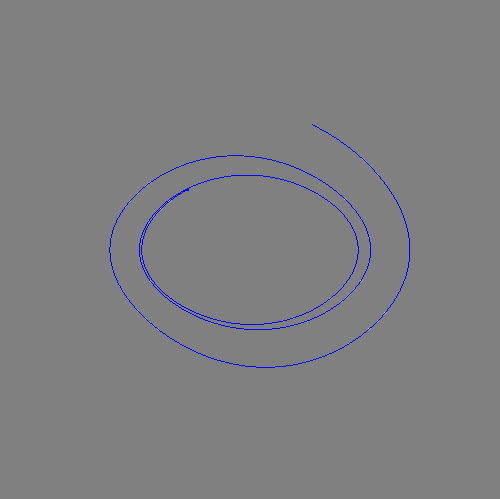
\includegraphics[width = 0.5\columnwidth]{pendolo_limite.png}
  \caption{Pendolo smorzato con forzante esterna nel caso di ciclo limite. $B = 0.5$, $Q= 0.5$ $\omega_{ext} = \tfrac{2}{3}$}
 \end{figure*}


Come detto precedentemente, si è risolto questo sistema newtoniano analiticamente non integrabile. L'equazione del moto è la seguente:
$$
  \ddot{\theta} \ = \ -sin(\theta) -Q \dot{\theta}+B cos(\omega_{ext} t)
$$
Che equivale al sistema newtoniano associato, ponendo $ x_1 = \theta $ e $x_2 = \dot{\theta}$.

In questo caso i coefficienti sono i seguenti:
\begin{align*}
B \ & = 0.5\\
Q & = 0.5 \\
\omega_{ext} &= \tfrac{2}{3}
\end{align*}
Questa scelta di coefficienti impedisce al sistema di uscire dall'intervallo $ -\tfrac{\pi}{2} \leq \theta \leq \tfrac{\pi}{2}$ e il sistema dopo un transiente iniziale,
si porta sull' orbita del ciclo limite.
Diverso è il caso in cui si aumenta il coefficiente della forzante:
\begin{align*}
B \ & = 0.3\\
Q & = 1.4 \\
\omega_{ext} &= \tfrac{2}{3}
\end{align*}
\begin{figure*}[!h]
\centering
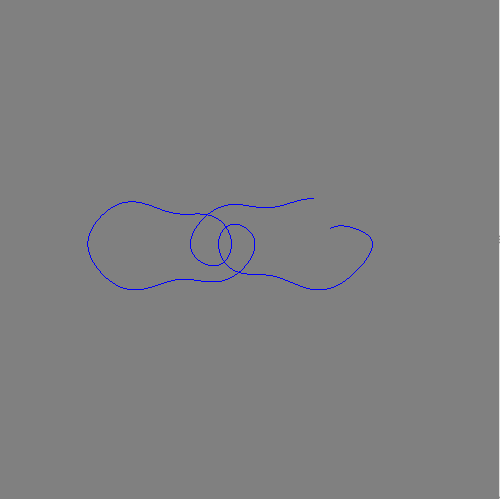
\includegraphics[width=0.7\columnwidth]{sovra1.png}
% \subfigure{\includegraphics[width=0.5\columnwidth]{Q=2_lungo.eps}}
 %\includegraphics[width=0.3\columnwidth]{B=3_lungo-lungo.eps}
\end{figure*}


\subsubsection{Oscillatore di van der Pol}
\begin{figure*}[!h]
  \centering
  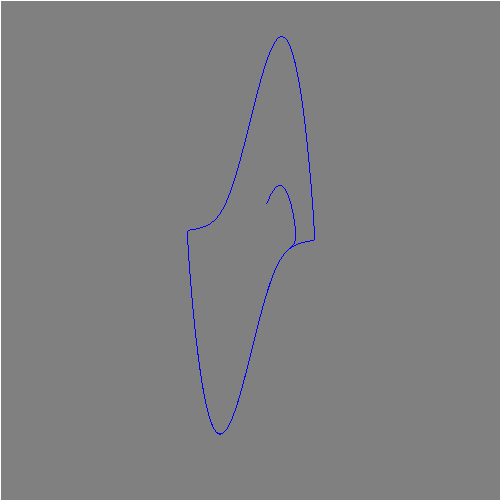
\includegraphics[width = 0.6\columnwidth]{van_der_pol.png}
  \caption{Oscillatore di van der Pol. Si può notare il ciclo limite}
\end{figure*}

Un'altro sistema studiato è l'oscillatore di \emph{van der Pol}.
$$
\frac{d^2x}{dt^2}-\mu(1-x^2)\frac{dx}{dt}+x = 0
$$
nella simulazione è stato posto $\mu = 4$.
\pagebreak
\section{Equazione di Schr\"{o}dinger}
L'equazione di Schr\"{o}dinger per una particella in un potenziale armonico è un problema molto più complicato dei precedenti già trattati.
In primo luogo si ha a che fare con equazioni differenziali alle derivate parziali invece che con equazioni differenziali ordinarie.
Inoltre, si passa da un sistema che ha un basso numero di gradi di libertà (nel caso precedente 2) a un sistema che (teoricamente) ha infiniti gradi di libertà.
Nella risoluzione di questo problema si è scelto di discretizzare lo spazio (bidimensionale in questo caso) e confinare il problema in una regione finita di spazio.
\subsection{Cenni teorici}
Nel nostro caso si è trattata l'equazione di Schr\"odinger indipendente dal tempo. L'hamiltoniana è quella ``standard'' bidimensionale.
$$
\mathcal{H} = \frac{\hat{p_x}^2+\hat{p_y}^2}{2m} + V(x,y) \quad \longrightarrow \quad i \p{}{t}\ket{\psi(t)} \ = \ \mathcal{H} \ket{\psi(t)}
$$
È noto che si può ricavare la soluzione dell'equazione come esponenziale dell'hamiltoniana:
$$
\ket{\psi(t)} = e^{ -i \mathcal{H} t} \ket{\psi(0)}
$$
La difficoltà però risiede nel calcolare l'esponenziale dell'hamiltoniana,tenendo presente che gli autovettori dell'hamiltoniana non sono noti.
\subsubsection{Algoritmo}
L'algoritmo consiste sostanzialmente nel cercare di risolvere l'equazione precedente, approssimando in maniera opportuna l'esponenziale.
In questo caso, abbiamo discretizzato lo spazio, creando un reticolo. È naturale ora associare alla funzione d'onda $ \braket{x,y}{\Psi(t)}$ una
matrice complessa. Ad ogni entrata della matrice corrisponderà il valore della funzione d'onda in quel punto del reticolo.\\
Si decide di approssimare l'esponenziale, usandone la definizio di sviluppo in serie, ma fermandosi ad un certo ordine. È possibile scegliere l'ordine a cui fermarsi nello sviluppo,
stimando l'autovalore massimo dell'hamiltoniana $ \lambda_{max}$. Così facendo, infatti si ha che:
$$
\left| exp \left( - i \mathcal{H} \delta t \right) - \sum_{i=0}^n \frac{\lambda_{max} \delta t)^{n}}{n!} \right| \ \simeq \frac{\left(\lambda_{max} \delta t\right)^{n+1}}{(n+1)!} 
$$
in questo modo, si può cercare un compromesso fra l'ordine dello sviluppo in serie e il valore del passo reticolare temporale $\delta t$.\\
Ad ogni passo dell'algoritmo, si calcola l'approssimazione di $ exp \left( -i \mathcal{H} \delta t \right)$ fino all'ordine desiderato e poi si
sostituisce $ \psi(t)$ con $\psi(t+\delta t) = exp \left( -i \mathcal{H} \delta t \right) \psi(t)$.
\subsubsection{Particella libera}
In questo caso l'hamiltoniana diventa semplicemente:
$$
\mathcal{H} = \frac{\hat{p_x}^2+\hat{p_y}^2}{2m}
$$
Nonostante si conoscano gli autovettori di questa hamiltoniana, si è analizzato questo problema anche per vagliare la correttezza dell'algoritmo.
Si è raggiunto un compromesso fra velocità dell'evoluzione della funzione d'onda e precisione dell'evoluzione, arrestando la serie all'ordine 25, con un $\delta t$ pari a 0.5.
Le unità di misura utilizzate nel sistema sono sostanzialmente arbitrarie, e sono state inglobate in una costante unica.
Le condizioni al contorno utilizzato sono di periodicità ai bordi.\\
Si è valutata inoltre l'unitarietà dell'operatore di evoluzione temporale ad ogni passo dell'algoritmo stampando su terminale il valore della norma
della matrice. La norma della funzione d'onda è stata inizialmente posta uguale ad uno. L'operatore di evoluzione temporale risulta unitario, nel senso che dopo una decina di minuti di simulazione,
la norma della funzione rimane inalterata: la norma differisce dall'unità a meno di fattori pari a $10^{-15/16}$. 

  \begin{figure*}[hp]
  \centering
    \subfigure[$\psi(0)$: il pacchetto è gaussiano e monocromatico, con momento diretto verticalmente verso il basso.]{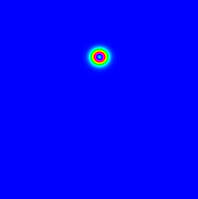
\includegraphics{free1.png}}
    \subfigure[Ora $\psi$ non ha più simmetria sferica. Si può notare lo ``spread'' del pacchetto.]{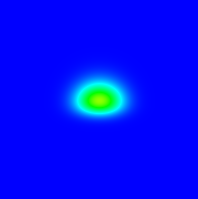
\includegraphics{free2.png}}
    \subfigure[Lo ``spread'' aumenta ancora. Si notano gli effetti delle condizioni al bordo]{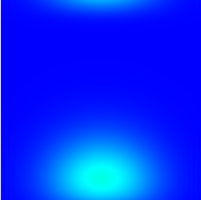
\includegraphics{free3.png}}
    \subfigure[La funzione d'onda inizia a intereferire con sè stessa.]{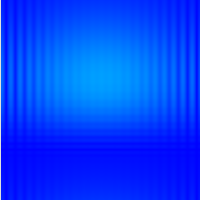
\includegraphics{free4.png}}
    \subfigure{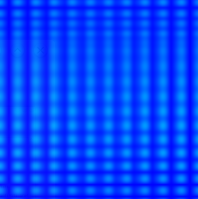
\includegraphics{free_crystal.png}}
    \subfigure{
\includegraphics{free5.png}}
    \caption{Evoluzione di un pacchetto gaussiano libero, con periodicità ai bordi.}
  \end{figure*}
  \pagebreak
\subsubsection{Muro di potenziale sferico}
In questo caso l'hamiltoniana utilizzata è quella completa, fornita all'inizio del capitolo. Anche in questo caso valgono le considerazioni precedenti e sono stati utilizzati gli stessi parametri di prima.
In questo caso il potenziale utilizzato è il seguente:
$$
V(x,y) \ = \ \begin{sistem}
              1 \quad \mbox{se} \quad  0< r < 10 \\
              0 \quad \mbox{altrimenti}
             \end{sistem}
$$
dove $r$ è il raggio dal centro della finestra ed è misurato in \emph{pixel} (o elemeti della matrice).

\begin{figure}[hp]
 \centering
 \subfigure[Pacchetto d'onda gaussiano distante dalla buca]{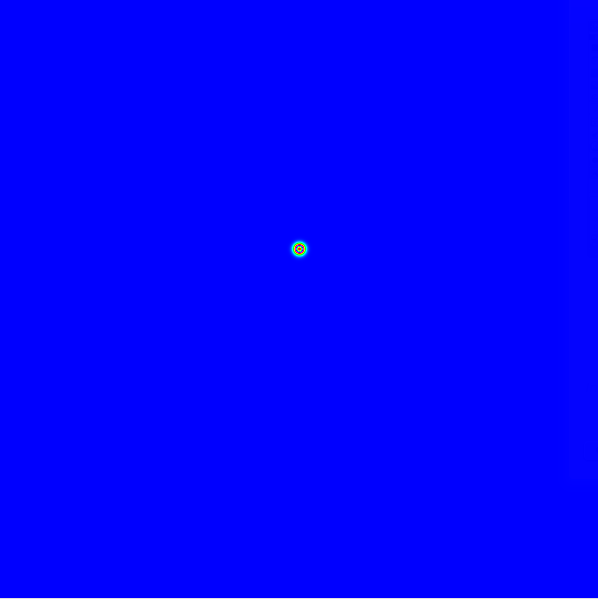
\includegraphics[width=0.4\columnwidth]{scattering1.png}}
 \subfigure[Pacchetto si scontra con la buca]{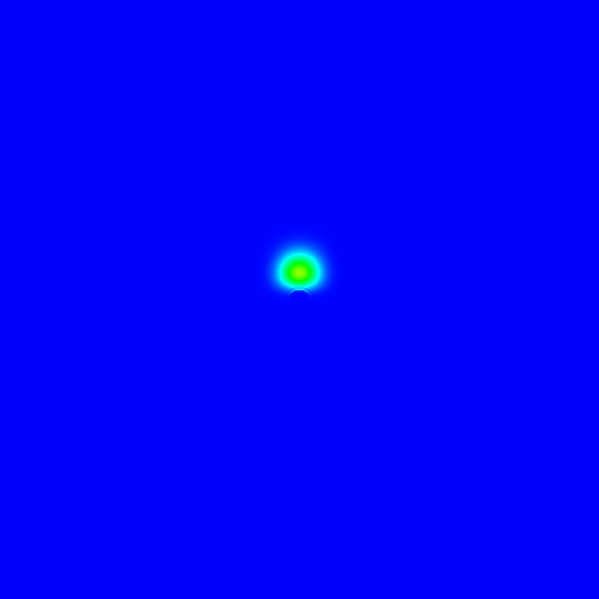
\includegraphics[width=0.4\columnwidth]{scattering2.png}}
 \caption{Scattering di un pacchetto gaussiano monocromatico con un muro di potenziale sferico.} 
 \end{figure}
 In questo caso, si intende visualizzare lo scattering del pacchetto d'onda contro questo potenziale sferico.
Per questo motivo, è stato necessario utilizzare un griglia più grande, rispetto a prima,
che passa da 200x200 a 600x600. Così facendo l'algoritmo diventa più lento di un fattore dieci circa.
Questa scelta è stata necessaria per poter
valutare l'andamento della funzione d'onda quando si è molto distanti dalla buca, in modo da poter considerarla ``all'infinito''. 
Ciò è dovuto anche alle condizioni al bordo utilizzate: utilizzando la periodicità al bordo, la funzione d'onda interferisce poco dopo lo scattering
con sè stessa. Inoltre, non è possibile diminuire le dimensioni del pacchetto e della buca, perchè così facendo,
gli errori di discretizzazione darebbero problemi.
\begin{figure}[h]
 \centering
 \subfigure{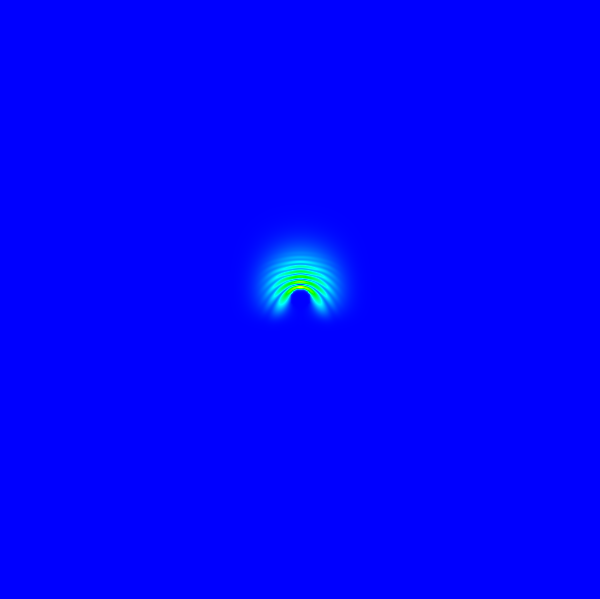
\includegraphics[width=0.4\columnwidth]{scattering3.png}}
 \subfigure{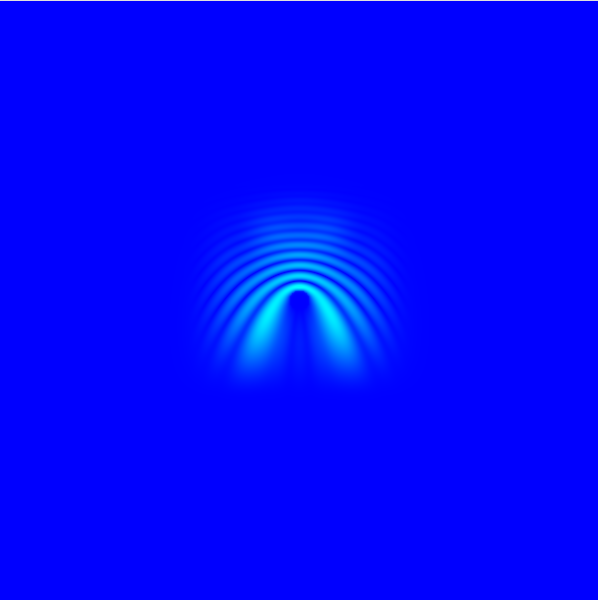
\includegraphics[width=0.4\columnwidth]{scattering4.png}}
 \subfigure{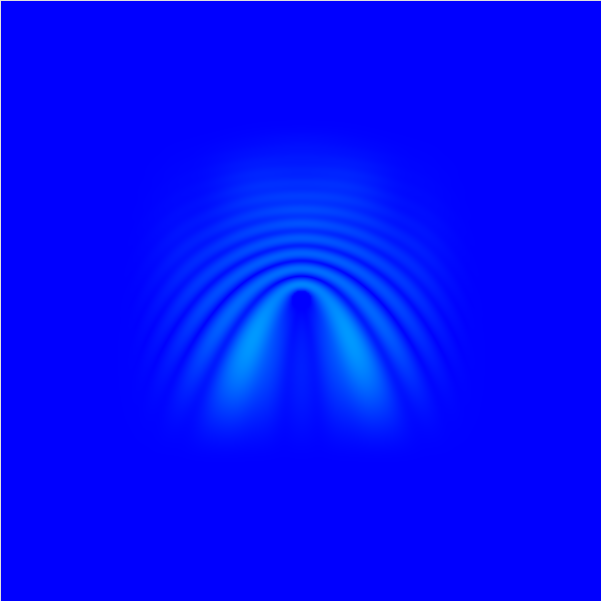
\includegraphics[width=0.4\columnwidth]{scattering5.png}}
 \caption{Scattering di un pacchetto gaussiano monocromatico con un muro di potenziale sferico.(continua)} 
 \end{figure}
\subsection{Buca di potenziale sferico}
Il problema è simile al caso precedente, ma ora trattiamo una buca di potenziale invece che un ``muro''.
$$
V(x,y) \ = \ \begin{sistem}
             -1 \quad \mbox{se} \quad  0< r < 20 \\
              0 \quad \mbox{altrimenti}
             \end{sistem}
$$
Inoltre, la griglia è stata ridotta da 600x600 a 500x500, per velocizzare la simulazione.
\begin{figure}[hp]
 \centering
 \subfigure{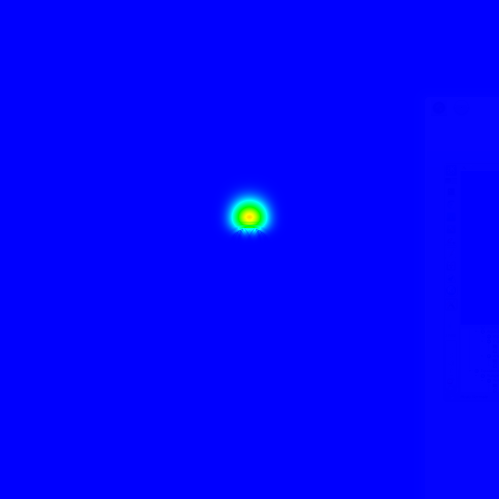
\includegraphics[width=0.4\columnwidth]{scattering_buca1.png}}
 \subfigure{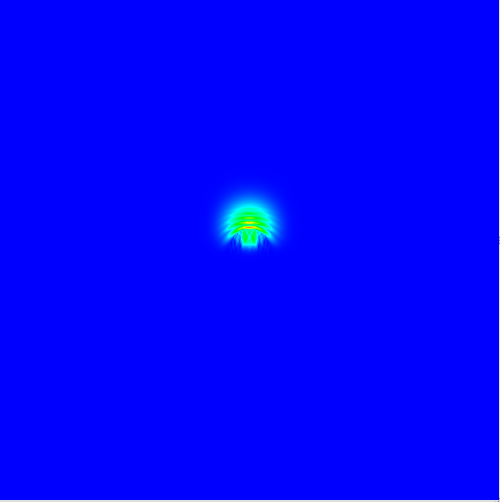
\includegraphics[width=0.4\columnwidth]{scattering_buca2.png}}
 \subfigure{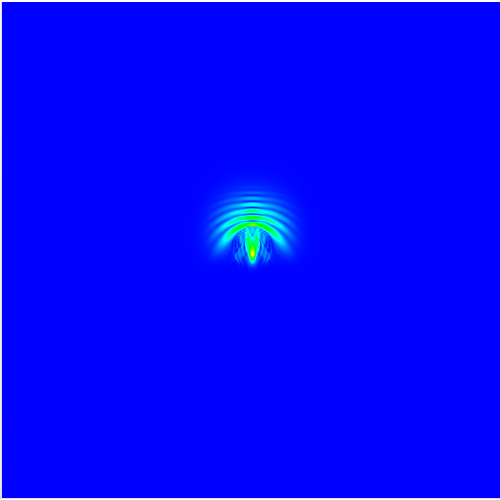
\includegraphics[width=0.4\columnwidth]{scattering_buca3.png}}
 \subfigure{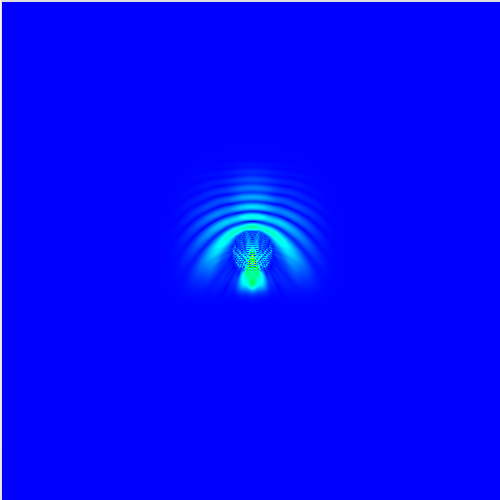
\includegraphics[width=0.4\columnwidth]{scattering_buca4.png}}
 \subfigure{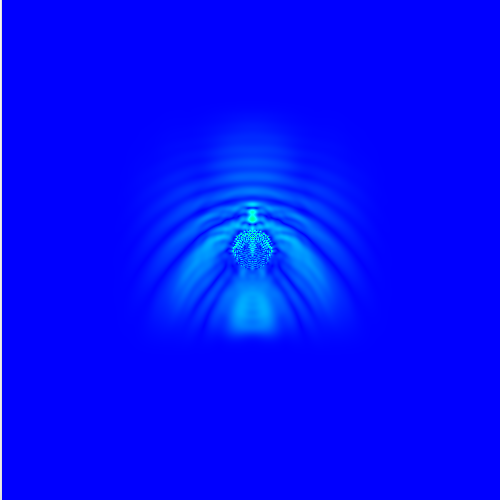
\includegraphics[width=0.4\columnwidth]{scattering_buca5.png}}
 \subfigure{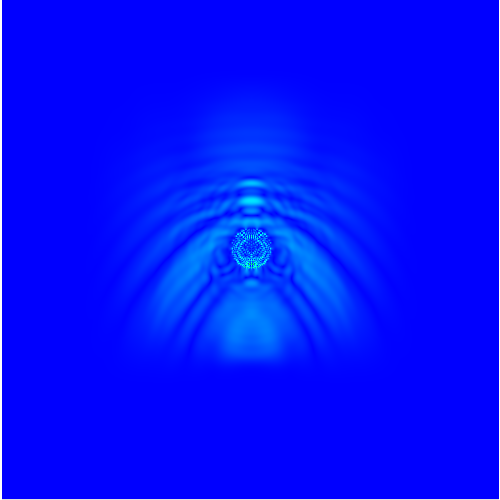
\includegraphics[width=0.4\columnwidth]{scattering_buca6.png}}
 \caption{Scattering di un pacchetto gaussiano monocromatico con una buca di potenziale sferico.} 
 \end{figure}
 \subsection{Effetto tunnel}
 Si studia il fenomeno dell'effetto tunnel analizzando il comportamento del sistema per una barriera di potenziale ``orizzontale'' di larghezza variabile.
 \subsubsection{Barriera larga}
 Si è cercato di studiare quantitativamente il fenomeno dell'effetto tunnel. Qualitativamente, perchè in questo caso non si conosce il valore dell'energia.
 D'altronde, è possibile studiare come varia la situazione modificando i parametri che entrano in gioco nell'effetto tunnel: l'altezza della barriera di potenziale e la larghezza della stessa.
 In entrambi i casi è stato fissato il potenziale a $1$, come nel caso dello scattering.
 La larghezza della barriera è stata posta uguale a 20 (nelle unità di misura del problema).
\begin{figure}[hp]
 \centering
 \subfigure{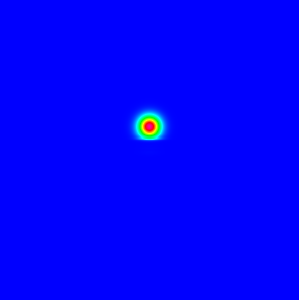
\includegraphics[width=0.4\columnwidth]{notunnel1.png}}
 \subfigure{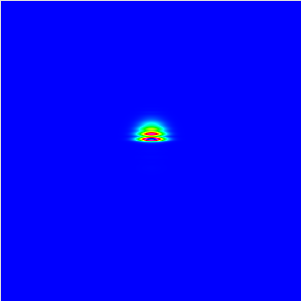
\includegraphics[width=0.4\columnwidth]{notunnel2.png}}
 \subfigure{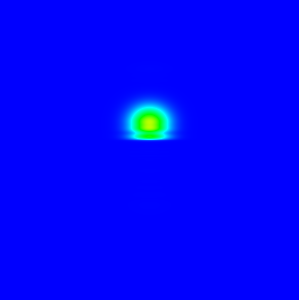
\includegraphics[width=0.4\columnwidth]{notunnel3.png}}
 \subfigure{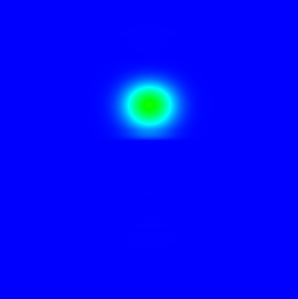
\includegraphics[width=0.4\columnwidth]{notunnel4.png}}
 \subfigure{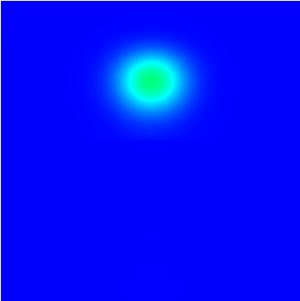
\includegraphics[width=0.4\columnwidth]{notunnel5.png}}
 \caption{Effetto tunnel contro una barrieri di potenziale larga 20.} 
 \end{figure}
 
 
 \subsubsection{Barriera stretta}
 In questo caso, si è accorciata la larghezza della barriera di potenziale. Ora esso è molto più stretta rispetto alle dimensioni spaziali del pacchetto d'onda.
 L'altezza della barriera è sempre pari a 1.
\begin{figure}[hp]
 \centering
 \subfigure{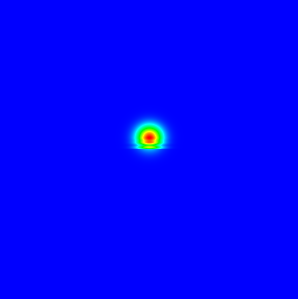
\includegraphics[width=0.4\columnwidth]{tunnel1.png}}
 \subfigure{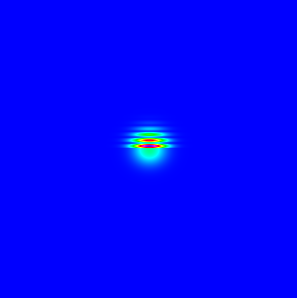
\includegraphics[width=0.4\columnwidth]{tunnel3.png}}
 \subfigure{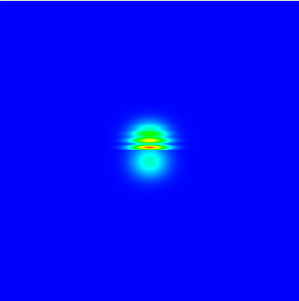
\includegraphics[width=0.4\columnwidth]{tunnel2.png}}
 \subfigure{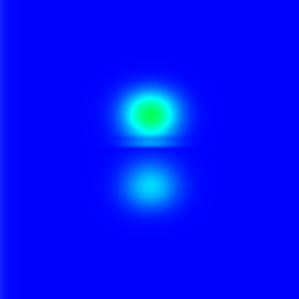
\includegraphics[width=0.4\columnwidth]{tunnel4.png}}
  \caption{Effetto tunnel contro una barrieri di potenziale larga 1.} 
 \end{figure}
 \subsection{Diffrazione da doppia fenditura}
 Questa parte mira a simulare l'esperimento della doppia fenditura, di grande importanza storica per lo sviluppo della meccanica quantistica.\\
 Per fare ciò si è inserita una barriera di potenziale molto alta ( $V = 100$) con due fenditure larghe 5. La barriera è stata posta orizzontalmente, come la barriera di potenziale nel caso dell'effetto tunnel.
 A causa del valore di $V$ è stato necessario eseguire molti più calcoli rispetto ai casi precedenti per avere una buona precisione. Infatti in questo caso
 è stato necessario porre $\delta t = 0.1$ (invece che $\delta t = 0.5 $ nei casi precedenti) e aumentare l'ordine dello sviluppo in serie fino a 30.
 Questo è causato proprio dal fatto che gli autovalori dell'hamiltoniana sono molto più elevati, a causa della barriera di potenziale.
\begin{figure}[hp]
 \centering
 \subfigure{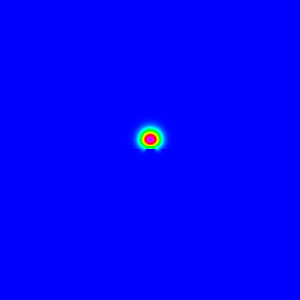
\includegraphics[width=0.4\columnwidth]{fenditura1.png}}
 \subfigure{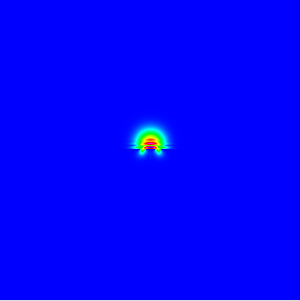
\includegraphics[width=0.4\columnwidth]{fenditura2.png}}
 \subfigure{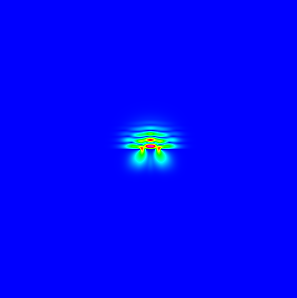
\includegraphics[width=0.4\columnwidth]{fenditura3.png}}
 \subfigure{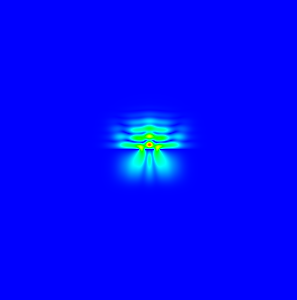
\includegraphics[width=0.4\columnwidth]{fenditura4.png}}
 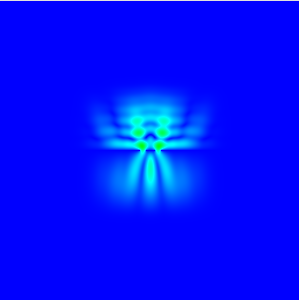
\includegraphics[width=0.5\columnwidth]{fenditura5.png}
 \caption{Diffrazione da una doppia fenditura.} 
 \end{figure}
 \subsection{Equazione del calore}
 Dopo aver risolto l'equazione di Schr\"{o}dinger si è deciso di risolvere anche l'equazione del calore, vista la notevole similitudine tra l'equazione di Schr\"{o}dinger nel caso libero
 e l'equazione del calore.
 \begin{align}
  \mbox{Schr\"{o}dinger libera} \qquad i \p{}{t} \psi(x,y,t) \ & = \ - a \ \nabla^2 \psi (x,y,t) \\
  \mbox{Equazione del calore} \qquad \p{}{t} \psi(x,y,t) \ & = \ - k \ \nabla^2 \psi (x,y,t)
 \end{align}
Come si può vedere l'unica differenza risiede nel fatto che l'equazione di Schr\"{o}dinger è complessa e ha una ``i'' insieme alla derivata temporale.
Ciò è proprio quello che permette alle soluzioni di avere un carattere ondulatorio, mentre l'equazione del calore produce soluzioni dal carattere diffusivo.
Inoltre, proprio per questo motivo, l'equazione del calore risulta molto più stabile rispetto all'equazione di Schr\"{o}dinger. Infatti, i parametri dell'algoritmo utilizzati questa volta sono:
$$
 N_{max} = 2 \qquad \delta t = 1 \qquad  
$$
 Per questo motivo, inoltre è stato possibile aumentare la dimensione del reticolo fino a 500x500, mantenendo la stessa velocità di esecuzione.
\end{document}